\documentclass{beamer}
\usepackage[utf8]{inputenc}

\usetheme{Madrid}
\usecolortheme{default}
\usepackage{color}
\usepackage{colortbl}

\usepackage{algorithmic}
\usepackage{listings}
\usepackage{hyperref}
\hypersetup{colorlinks=true,urlcolor=blue}

\begin{document}
	
\title{Proximal Policy Optimization (PPO)} 
\author{Fabrício Barth}
\institute{Insper Instituto de Ensino e Pesquisa}
\date{Maio de 2023}
	
\maketitle

\def\HiLi{\leavevmode\rlap{\hbox to \hsize{\color{yellow!50}\leaders\hrule height .8\baselineskip depth .5ex\hfill}}}
	
\def\TA{\leavevmode\rlap{\hbox to \hsize{\color{cyan!50}\leaders\hrule height .8\baselineskip depth .5ex\hfill}}}

\def\TB{\leavevmode\rlap{\hbox to \hsize{\color{red!50}\leaders\hrule height .8\baselineskip depth .5ex\hfill}}}
	
\begin{frame}{Contexto}
\begin{itemize}
	\item Na última aula vimos o funcionamento do algoritmo \textbf{Reinforce}. 
	\item O algoritmo \textbf{Reinforce} tem um problema relacionado com a atualização dos parâmetros do modelo. 
	\item Dependendo do espaço de busca do problema, a atualização dos parâmetros pode ser grande demais e levar para situações indesejadas. Mesmo em situações onde a atualização dos parâmetros estava levando para uma situação de otimização. 
\end{itemize}
\end{frame}

\begin{frame}{Proximal Policy Optimization (PPO)}
	\begin{itemize}
		\item O PPO é um método de \textit{policy gradient} que evita a atualização grande dos parâmetros da \textit{policy}.
		\item Basicamente, o PPO usa uma razão entre a política atual e a política antiga e mantêm esta razão entre $\left[ 1 - \epsilon, 1 + \epsilon \right]$.
		\item Desta forma o algoritmo PPO garante que a atualização do parâmetros não seja tão grande e o treinamento se torna mais estável. 
	\end{itemize}
	
	
\end{frame}
	
\begin{frame}{Objetivo desta aula}
	Ao final desta aula, você será capaz de compreender como funciona e como implementar o algoritmo \textbf{PPO}.
\end{frame}

\begin{frame}{Algoritmo Reinforce}
	\begin{algorithmic} 
		\STATE \emph{\textbf{function} REINFORCE($\alpha$, $\gamma$, episódios):}
		\STATE inicializar os valores de $\theta$ para a policy $\pi(A|S,\theta)$ arbitrariamente
		\FOR {todos os episódios}
		\STATE gerar um episódio ${s_{0},a_{0},r_{1},\cdots,s_{T-1},a_{T-1},r_{T}}$ seguindo $\pi(.|.,\theta)$
		\FOR {cada passo dentro do episódio $t = 0, 1, 2, \cdots, T-1$}
			\STATE $G \leftarrow \sum_{k=t+1}^{T} \gamma^{k-t-1} \times r_{k}$
			\STATE $\theta \leftarrow \theta + \alpha \times \bigtriangledown \log \pi(a_{t}|s_{t}, \theta) \times G$
		\ENDFOR
		\ENDFOR
	\end{algorithmic}
\end{frame}

\begin{frame}{Equação central}
	A equação central do algoritmo \textsc{Reinforce} é: 
	
	\begin{equation}
		\theta \leftarrow \theta + \alpha \times \bigtriangledown \log \pi(a_{t}|s_{t}, \theta) \times G
	\end{equation}

	que também pode ser escrita como: 
	
	\begin{equation}
		L^{PG}(\theta) = \hat{E} \left[ \log \pi_{\theta}(a_{t}|s_{t}).\hat{G}(s_{t},a_{t}) \right]
	\end{equation}
\end{frame}

\begin{frame}{Estimador de vantagem}
	Schulman,2015, propõe o uso do conceito de \textit{advantage estimation} ou estimador de vantagem no lugar do \textit{discounted rewards} $\hat{G}(s_{t},a_{t})$. 
	
	\begin{equation}
	L^{PG}(\theta) = \hat{E} \left[ \log \pi_{\theta}(a_{t}|s_{t}).\hat{A}(s_{t},a_{t}) \right]
	\end{equation}	
	
	onde: 
	
	\begin{equation}
		\hat{A}(s_{t},a_{t}) = \hat{Q}(s_{t},a_{t}) - \hat{V}(s_{t})
	\end{equation}

\begin{itemize}
	\item $\hat{Q}(s_{t},a_{t})$ é o \textit{discounted rewards}, e;
	\item $\hat{V}(s_{t})$ é a função baseline.
\end{itemize}	

\end{frame}


\begin{frame}{Estimador de vantagem}
\begin{eqnarray}
	\hat{A}(s_{t},a_{t}) = \hat{Q}(s_{t},a_{t}) - \hat{V}(s_{t}) \nonumber \\
	\hat{Q}(s_{t},a_{t}) = \sum_{k=t+1}^{T} \gamma^{k-t-1} \times r_{k} \nonumber \\
	\hat{V}(s_{t}) = \sum_{a_{t} \in A} \pi (a_{t}|s_{t}).\hat{Q}(s_{t},a_{t}) \nonumber \\
	\hat{A}(s_{t},a_{t}) = \hat{Q}(s_{t},a_{t}) - \sum_{a_{t} \in A} \pi (a_{t}|s_{t}).\hat{Q}(s_{t},a_{t}) 
\end{eqnarray}	
\end{frame}


\begin{frame}{Razão entre políticas}
	
	Schulman, 2017, propõe o uso da razão entre a política atual e a política antiga: 
	
	\begin{eqnarray}
	L^{TRPO}(\theta) = \hat{E} \left[\frac{\pi_{\theta}(a_{t}|s_{t})}{\pi_{\theta old}(a_{t}|s_{t})}.\hat{A}(s_{t},a_{t}) \right] = \hat{E}  \left[ r(\theta). \hat{A}(s_{t},a_{t}) \right] \\	
	r(\theta) = \frac{\pi_{\theta}(a_{t}|s_{t})}{\pi_{\theta old}(a_{t}|s_{t})} 
	\end{eqnarray}


\begin{itemize}
	\item Lembrando que $\pi_{\theta}(a_{t}|s_{t})$ representa a probabilidade de $a_{t}$ acontecer em $s_{t}$.
	\item Sendo assim, se $r(\theta) < 1$ então $a_{t}$ tem uma probabilidade maior de ocorrer em $\theta old$ do que em $\theta$.
	\item Se $r(\theta) > 1$ então $a_{t}$ tem uma probabilidade maior de ocorrer na política atual do que na antiga. 
\end{itemize}

\end{frame}


\begin{frame}{Mas e se $r(\theta)$ for um número muito maior que 1? .. 100?}
	
O algoritmo PPO define uma nova função objetivo que garante que a política nova não fique muito longe da política antiga:
	
	\begin{equation}
	L^{CLIP}(\theta) = \hat{E} \left[ \min \left(r(\theta).\hat{A}(s_{t},a_{t}) , clip(r(\theta), 1 - \epsilon, 1 + \epsilon).\hat{A}(s_{t},a_{t}) \right) \right]		
	\end{equation}

\begin{itemize}
	\item Com esta função \textsc{CLIP}, nós temos duas possibilidades de $r(\theta)$, a versão original (não limitada) e a versão limitada onde o limite é entre $\left[ 1 - \epsilon, 1 + \epsilon \right]$, onde $\epsilon$ é um hiperparâmetro que nos ajuda a definir os limites. 
	\item No artigo de Schulman, 2017 é utilizado o valor 0.2 para $\epsilon$.
\end{itemize}
	
\end{frame}


\begin{frame}{Função objetiva "clipped"}
	Esta função não permite que atualizações na política sejam feitas quando a razão ($r(\theta)$) entre a política atual e a antiga fica fora da "zona de conforto". 
	\begin{center}
		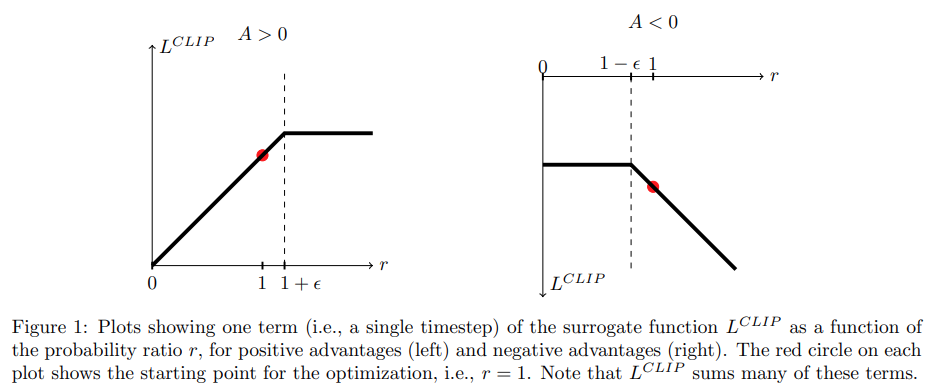
\includegraphics[width=1\textwidth]{img/clip.png}
	\end{center}
\end{frame}

\begin{frame}{Algoritmo PPO, estilo "Actor-Critic"}

\begin{algorithmic} 
	\FOR {iterações=1,2,$\cdots$}
		\FOR {actor=1,2,$\cdots$, N}
			\STATE gerar um episódio ${s_{0},a_{0},r_{1},\cdots,s_{T-1},a_{T-1},r_{T}}$ seguindo $\pi(.|.,\theta_{old})$
			\STATE calcular as estimativas de vantagem $\hat{A}_{1}, \cdots, \hat{A}_{T}$
		\ENDFOR
	
	\STATE Otimiza $L^{CLIP}(\theta)$ com $K$ épocas e minibatch com tamanho $M \leq NT$. 
	\STATE $\theta_{old} \leftarrow \theta$
	
	\ENDFOR
\end{algorithmic}	
	
\end{frame}


\begin{frame}{Algoritmo PPO, estilo "Actor-Critic"}
	
	\begin{algorithmic} 
		\FOR {iterações=1,2,$\cdots$}
		\FOR {actor=1,2,$\cdots$, N}
		\STATE \TA gerar um episódio ${s_{0},a_{0},r_{1},\cdots,s_{T-1},a_{T-1},r_{T}}$ seguindo $\pi(.|.,\theta_{old})$
		\STATE \TA calcular as estimativas de vantagem $\hat{A}_{1}, \cdots, \hat{A}_{T}$
		\ENDFOR
		
		\STATE \TB Otimiza $L^{CLIP}(\theta)$ com $K$ épocas e minibatch com tamanho $M \leq NT$. 
		\STATE \TB $\theta_{old} \leftarrow \theta$
		
		\ENDFOR
	\end{algorithmic}	

Este algoritmo é dividido em duas threads: 

\begin{itemize}
	\item atores: responsáveis por gerar os episódios e calcular toda a sequência de $S, A, R, \hat{A}$ com base na policy vigente.
	\item críticos: responsáveis por otimizar os valores da policy. 
\end{itemize}
	
\end{frame}


\begin{frame}{Algoritmo PPO, estilo "Actor-Critic"}
	
	\begin{algorithmic} 
		\FOR {iterações=1,2,$\cdots$}
		\FOR {actor=1,2,$\cdots$, N}
		\STATE \TA gerar um episódio ${s_{0},a_{0},r_{1},\cdots,s_{T-1},a_{T-1},r_{T}}$ seguindo $\pi(.|.,\theta_{old})$
		\STATE \TA calcular as estimativas de vantagem $\hat{A}_{1}, \cdots, \hat{A}_{T}$
		\ENDFOR
		
		\STATE Otimiza $L^{CLIP}(\theta)$ com $K$ épocas e minibatch com tamanho $M \leq NT$. 
		\STATE $\theta_{old} \leftarrow \theta$
		
		\ENDFOR
	\end{algorithmic}	
	
	Algumas observações: 
	
	\begin{itemize}
		\item $T$ não necessáriamente é um estado terminal. $T$ define o limite da trajetória. 
		\item a geração dos episódios acontece por $N$ atores independentes e paralelos.
	\end{itemize}
	
\end{frame}

\begin{frame}{Algoritmo PPO, estilo "Actor-Critic"}
	
	\begin{algorithmic} 
		\FOR {iterações=1,2,$\cdots$}
		\FOR {actor=1,2,$\cdots$, N}
		\STATE gerar um episódio ${s_{0},a_{0},r_{1},\cdots,s_{T-1},a_{T-1},r_{T}}$ seguindo $\pi(.|.,\theta_{old})$
		\STATE calcular as estimativas de vantagem $\hat{A}_{1}, \cdots, \hat{A}_{T}$
		\ENDFOR
		
		\STATE \TB Otimiza $L^{CLIP}(\theta)$ com $K$ épocas e minibatch com tamanho $M \leq NT$. 
		\STATE \TB $\theta_{old} \leftarrow \theta$
		
		\ENDFOR
	\end{algorithmic}	
	
	Algumas observações: 
	
	\begin{itemize}
		\item Tempos em tempos, a thread para atualização da policy dispara um Stochastic Gradient Descent sobre a função $L^{CLIP}(\theta)$. 
		\item executar treinamentos usando minibatch e com $K$ épocas não é usual em Reinforcement Learning. No entanto, devido ao uso da função $L^{CLIP}$ isso é possível.  
	\end{itemize}
	
\end{frame}


\begin{frame}{Usando a biblioteca stable\_baselines3}
	A biblioteca \textbf{stable\_baselines3} é um conjunto de implementações de algoritmos de Reinforcement Learning em pytorch: \href{https://stable-baselines3.readthedocs.io/en/master/}{https://stable-baselines3.readthedocs.io/en/master/} 
	
	\tiny
	\lstinputlisting[language=Python]{src/ppo.py}
\end{frame}

	
\begin{frame}{Referências}
	
	\small
	\begin{itemize}
		
		\item The 37 Implementation Details of Proximal Policy Optimization. Disponível \href{https://iclr-blog-track.github.io/2022/03/25/ppo-implementation-details/}{https://iclr-blog-track.github.io/2022/03/25/ppo-implementation-details/}. Último acesso em maio de 2023. 
		
		\item Schulman J, Levine S, Abbeel P, Jordan M, Moritz P. Trust region policy optimization. In International conference on machine learning 2015 Jun 1 (pp. 1889-1897). PMLR.v \href{https://doi.org/10.48550/arXiv.1502.05477}{https://doi.org/10.48550/arXiv.1502.05477}
		
		\item Schulman J, Wolski F, Dhariwal P, Radford A, Klimov O. Proximal policy optimization algorithms. arXiv preprint arXiv:1707.06347. 2017 Jul 20.
		
		\item Understanding Proximal Policy Optimization (Schulman et al., 2017). Disponível \href{https://blog.tylertaewook.com/post/proximal-policy-optimization}{blog.tylertaewook.com/post/proximal-policy-optimization}. Último acesso em maio de 2023. 
		
		\item Simonini, T. Proximal Policy Optimization (PPO). Unit 8, of the Deep Reinforcement Learning Class with Hugging Face. Disponível em \href{https://huggingface.co/blog/deep-rl-ppo}{https://huggingface.co/blog/deep-rl-ppo}. Último acesso em maio de 2023.
	\end{itemize}
\end{frame}
		
\end{document}
	
